\documentclass[tikz,border=2pt]{standalone}
\usepackage{tikz}
\usetikzlibrary{arrows.meta,calc}

\definecolor{roadgray}{RGB}{211,214,216}
\definecolor{curbdark}{RGB}{86,91,94}
\definecolor{curblight}{RGB}{139,145,148}
\definecolor{egocolor}{RGB}{65,145,162}
\definecolor{targetcolor}{RGB}{232,112,58}
\definecolor{nominalcolor}{RGB}{0,139,151}

\def\vehicleDrawingScale{0.44}
% Shared vector sedan, facing local +x. Arguments: center, yaw, color, steer.
% The caller defines vehicleDrawingScale; body envelope remains 2.10 x 0.96.
% Styling is illustrative, not a change to the vehicle model or dimensions.
\newcommand{\drawvehicle}[4]{%
    \begin{scope}[shift={(#1)},rotate=#2,scale=\vehicleDrawingScale,
        line join=round,line cap=round]
        \tikzset{carOutline/.style={draw=black!78,line width=0.48pt},
            carDetail/.style={draw=black!55,line width=0.26pt},
            carGlass/.style={carDetail,fill=white!80!#3}}
        % Four separate tires; the front pair follows the steering angle.
        \foreach \wheelY in {-0.515,0.515} {
            \begin{scope}[shift={(-0.515,\wheelY)}]
                \path[fill=black,draw=black,line width=0.25pt,
                    rounded corners=0.5pt] (-0.215,-0.085) rectangle (0.215,0.085);
            \end{scope}
            \begin{scope}[shift={(0.515,\wheelY)},rotate=#4]
                \path[fill=black,draw=black,line width=0.25pt,
                    rounded corners=0.5pt] (-0.215,-0.085) rectangle (0.215,0.085);
            \end{scope}
        }
        % Rounded bumper ends and gently tapered front/rear quarters.
        \path[carOutline,fill=white!40!#3]
            (-1.05,-0.28) .. controls (-1.05,-0.40) and (-0.94,-0.46) .. (-0.79,-0.47)
            .. controls (-0.30,-0.48) and (0.45,-0.48) .. (0.79,-0.45)
            .. controls (0.98,-0.43) and (1.05,-0.32) .. (1.05,-0.18)
            -- (1.05,0.18)
            .. controls (1.05,0.32) and (0.98,0.43) .. (0.79,0.45)
            .. controls (0.45,0.48) and (-0.30,0.48) .. (-0.79,0.47)
            .. controls (-0.94,0.46) and (-1.05,0.40) .. (-1.05,0.28) -- cycle;
        % Hood and trunk seams, with separate bumper lines.
        \draw[carDetail] (0.48,-0.35) .. controls (0.67,-0.38) and (0.86,-0.35) .. (0.94,-0.26)
            .. controls (0.98,-0.12) and (0.98,0.12) .. (0.94,0.26)
            .. controls (0.86,0.35) and (0.67,0.38) .. (0.48,0.35);
        \draw[carDetail] (-0.72,-0.36) -- (-0.92,-0.30)
            .. controls (-0.98,-0.12) and (-0.98,0.12) .. (-0.92,0.30) -- (-0.72,0.36);
        \draw[carDetail] (1.01,-0.15) -- (1.01,0.15);
        \draw[carDetail] (-1.01,-0.23) -- (-1.01,0.23);
        % Front and rear windscreens surround the central roof panel.
        \path[carGlass] (0.19,-0.29) .. controls (0.26,-0.17) and (0.26,0.17) .. (0.19,0.29)
            -- (0.44,0.36) .. controls (0.57,0.18) and (0.57,-0.18) .. (0.44,-0.36) -- cycle;
        \path[carGlass] (-0.45,-0.29) -- (-0.45,0.29) -- (-0.69,0.35)
            .. controls (-0.77,0.16) and (-0.77,-0.16) .. (-0.69,-0.35) -- cycle;
        \path[carDetail,fill=white!60!#3,rounded corners=0.8pt]
            (-0.43,-0.28) -- (0.17,-0.28) -- (0.17,0.28) -- (-0.43,0.28) -- cycle;
        % Side glazing, pillars, door seams, mirrors and lights are symmetric.
        \foreach \side in {-1,1} {
            \begin{scope}[yscale=\side]
                \path[carGlass] (-0.66,0.39) -- (-0.43,0.32) -- (-0.13,0.32)
                    -- (-0.13,0.41) -- cycle;
                \path[carGlass] (-0.08,0.32) -- (0.18,0.32) -- (0.41,0.39)
                    -- (-0.08,0.41) -- cycle;
                \draw[carDetail] (-0.10,0.42) -- (-0.10,0.47);
                \draw[carDetail] (-0.53,0.42) -- (-0.57,0.47);
                \draw[carDetail] (0.34,0.42) -- (0.31,0.47);
                \draw[carDetail] (-0.27,0.445) -- (-0.20,0.445);
                \draw[carDetail] (0.12,0.445) -- (0.19,0.445);
                \path[carDetail,fill=white!60!#3] (0.32,0.43) -- (0.32,0.56)
                    .. controls (0.34,0.61) and (0.43,0.59) .. (0.45,0.55)
                    -- (0.41,0.44) -- cycle;
                \path[carDetail,fill=white] (0.83,0.38) -- (0.96,0.28)
                    -- (0.96,0.19) .. controls (0.90,0.22) and (0.85,0.28) .. (0.83,0.38);
                \path[carDetail,fill=#3!65] (-0.95,0.30) -- (-0.83,0.39)
                    -- (-0.91,0.40) -- (-1.00,0.32) -- cycle;
            \end{scope}
        }
    \end{scope}%
}


\begin{document}
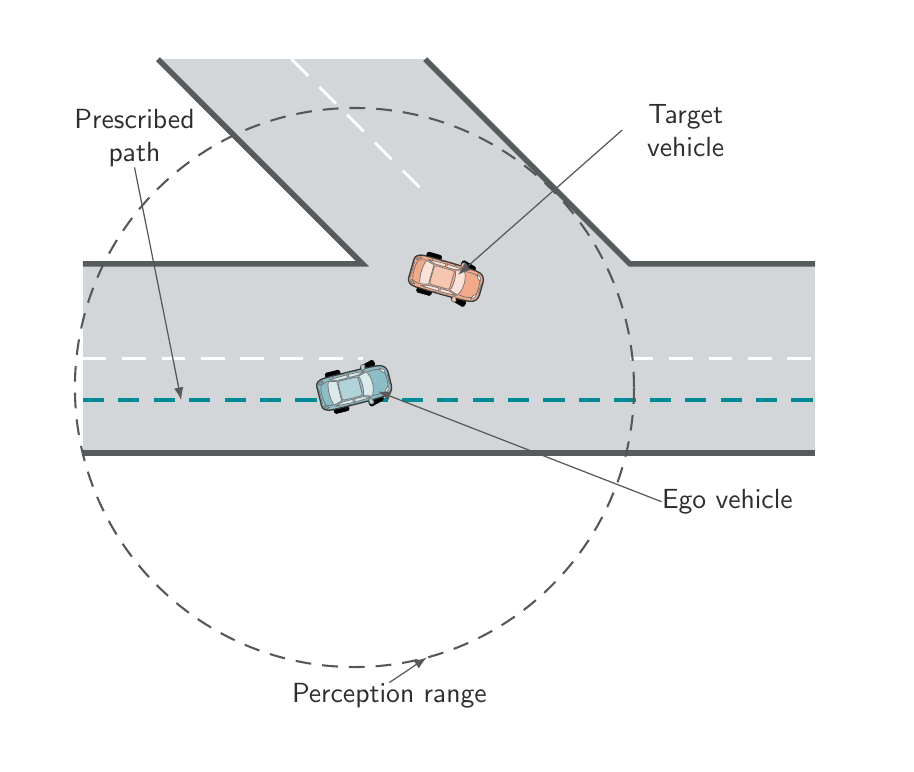
\begin{tikzpicture}[
    callout/.style={font=\sffamily\normalsize,align=center,text=black!82,inner sep=0pt},
    leader/.style={-{Latex[length=1.6mm,width=1.2mm]},draw=black!65,line width=0.45pt}
]
% Visual QA: manually passed. The automated title-band detector mistakes
% the two-line path callout for a title; this diagram has no title band.
% Design critique: keep. Math/diagram logic review: schematic.
% Exact invariants: Fig. 3 body/wheel angles, equal road widths,
% ego-centered sensing, and an ego footprint within its travel lane.
% Relative centers start from Fig. 3 at scale 0.44; the target is shifted
% slightly downward so its body straddles the side-road mouth.
% The branch is placed around the target in its inbound right-hand lane.
\path[use as bounding box] (-5.45,-4.90) rectangle (5.45,4.20);
\def\egoHeading{14}
\def\targetHeading{-16}
\def\egoSteer{15}
\def\targetSteer{-15}
\def\laneCenterY{-0.53}
\def\roadHalfWidth{1.20}
\def\branchHeading{-45}
\def\branchMouthX{0.50}
\def\branchTopY{3.80}
\def\sensingradius{3.55}
% The ego is displaced toward the lane centerline while keeping its Fig. 3
% heading. Its center does not coincide with the nominal reference path.
\def\egoLateralOffset{0.16}
% Translate both vehicles together; the target and sensing circle follow ego.
\def\vehicleRightShift{0.35}
\coordinate (egoVehicle) at ({-1.65+\vehicleRightShift},{\laneCenterY+\egoLateralOffset});

% The branch and main road have equal perpendicular width, 2*roadHalfWidth.
\pgfmathsetmacro{\branchHalfMouth}{\roadHalfWidth/abs(sin(\branchHeading))}
\pgfmathsetmacro{\branchLeftMouth}{\branchMouthX-\branchHalfMouth}
\pgfmathsetmacro{\branchRightMouth}{\branchMouthX+\branchHalfMouth}
\pgfmathsetmacro{\branchTopX}{\branchMouthX+(\branchTopY-\roadHalfWidth)/tan(\branchHeading)}
\pgfmathsetmacro{\branchLeftTop}{\branchTopX-\branchHalfMouth}
\pgfmathsetmacro{\branchRightTop}{\branchTopX+\branchHalfMouth}

% Fig. 3 centers: ego (3.75,1.35), target (6.40,5.40).
% Translate the scaled displacement to the off-reference ego center, then
% lower the target by 0.40 drawing units while keeping its rear part in the branch.
\pgfmathsetmacro{\relativeX}{0.44*(6.40-3.75)}
\def\targetDownwardShift{0.40}
\pgfmathsetmacro{\relativeY}{0.44*(5.40-1.35)-\targetDownwardShift}
\coordinate (targetVehicle) at ($(egoVehicle)+(\relativeX,\relativeY)$);

\path[fill=roadgray] (-4.75,-\roadHalfWidth) rectangle (4.55,\roadHalfWidth);
\path[fill=roadgray] (\branchLeftMouth,\roadHalfWidth) -- (\branchRightMouth,\roadHalfWidth)
    -- (\branchRightTop,\branchTopY) -- (\branchLeftTop,\branchTopY) -- cycle;
\draw[curbdark,line width=2.0pt] (-4.75,-\roadHalfWidth) -- (4.55,-\roadHalfWidth);
\draw[curbdark,line width=2.0pt] (-4.75,\roadHalfWidth) -- (\branchLeftMouth,\roadHalfWidth)
    -- (\branchLeftTop,\branchTopY);
\draw[curbdark,line width=2.0pt] (\branchRightTop,\branchTopY)
    -- (\branchRightMouth,\roadHalfWidth) -- (4.55,\roadHalfWidth);
% Center markings stop before the open intersection.
\draw[white,line width=1.0pt,dash pattern=on 3mm off 2mm]
    (-4.75,0) -- (\branchLeftMouth,0);
\draw[white,line width=1.0pt,dash pattern=on 3mm off 2mm]
    (\branchRightMouth,0) -- (4.55,0);
\draw[white,line width=1.0pt,dash pattern=on 3mm off 2mm]
    (\branchTopX,\branchTopY) -- ($(\branchMouthX,\roadHalfWidth)+(135:1.20)$);
% Prescribed reference path, distinct from the instantaneous ego pose.
\draw[nominalcolor,line width=1.25pt,dash pattern=on 2.7mm off 1.8mm]
    (-4.75,\laneCenterY) -- (4.55,\laneCenterY);
\draw[draw=black!66,line width=0.75pt,dash pattern=on 2mm off 1.4mm]
    (egoVehicle) circle[radius=\sensingradius];
\drawvehicle{egoVehicle}{\egoHeading}{egocolor}{\egoSteer}
\drawvehicle{targetVehicle}{\targetHeading}{targetcolor}{\targetSteer}

\node[callout,anchor=west,text width=16mm] (targetLabel) at (2.10,2.90) {Target\\vehicle};
\draw[leader] (targetLabel.west) -- ($(targetVehicle)+(0.15,0.05)$);
\node[callout,anchor=west] (egoLabel) at (2.60,-1.82) {Ego vehicle};
\draw[leader] (egoLabel.west) -- ($(egoVehicle)+(0.30,-0.05)$);
\node[callout,anchor=west,text width=16mm] (pathLabel) at (-4.90,2.80) {Prescribed\\path};
\draw[leader] (pathLabel.south) -- (-3.50,\laneCenterY);
\node[callout,anchor=west] (rangeLabel) at (-2.10,-4.28) {Perception range};
\draw[leader] (rangeLabel.north) -- ($(egoVehicle)+(285:\sensingradius)$);
\end{tikzpicture}
\end{document}
